\section{Strategic manipulation of the ED-EMS interface} \label{sec:model_overview}

The problem studied is a 3-player normal form game. The players are:
  
\begin{itemize}
    \item the decision makers of two Emergency Departments (EDs)
    \item the Emergency Medical Services (EMS) that distribute individuals in 
    ambulances to the EDs
\end{itemize}

This is a standard normal form game~\cite{Maschler2013},  
in that each player in this game has their own objectives which they aim to 
optimise.
More specifically, the EDs' objective is captured by an upper bound
of the time that a fixed proportion of individuals spend in the system, 
while the EMS aims to minimise the time that its ambulances 
are blocked.
This can be generalised for any such system where instead of EDs there are some
queueing systems and instead of the EMS there is some distributor that allocates
individuals to the queueing systems.

The parameters of the model correspond to the following parameters of the ED 
and the EMS:

\begin{itemize}
    \item \( \lambda_2 \): The rate of non-emergency patients that the EMS 
    receives and distributes to EDs
    % TODO: Use consistent notation of non-urgent/non-emergency patients
    \item \( \lambda_{1_i} \): The arrival rate of other patients to ED 
    \(i\in\{A, B\}\)
    \item \( \mu_i \): The service rate of patients at ED \(i\in\{A, B\}\)
    \item \( C_i \): The number of available resources (healthcare 
    professionals) in the ED \(i\in\{A, B\}\)
    % TODO: Make sure that servers are defined the same way throughout
    \item \( T_i \): The action that ED \(i\in\{A, B\} \) chooses to play which 
    corresponds to the threshold at which they do not accept EMS patients.
    \item \( N_i \): The total patient capacity of the ED \(i\in\{A, B\} \)
    \item \( M_i \): The total parking capacity of the ED \(i\in\{A, B\} \)
    \item \( t \): The time target for both EDs
    \item \( \alpha \in [0, 1] \) : Weighted average of blocking time and 
    lost individuals (equation \ref{eq:obj_distributor})
\end{itemize}

The strategies of the two EDs are the range of thresholds that they can choose
from and their utilities is the proportion of individuals whose time in the 
system is within a predetermined target time.
The EMS has to decide how to distribute its patients among the two EDs so that 
the weighted combination of the ambulance blocking time and the percentage of 
lost ambulances is minimised. 
This can be illustrated by figure \ref{fig:diagram_of_game_theoretic_model}.
The interaction between the two
EDs is a normal form game that is then used to inform the decision of the EMS.
Note that the formulated game here assumes that prior to making a choice the 
EMS knows the strategies that each ED is playing (figure 
\ref{fig:imperfect_info_game}). 
This corresponds to reacting to experienced delays.


\begin{figure}[H]    
    \centering
    \begin{minipage}{.25\textwidth}
        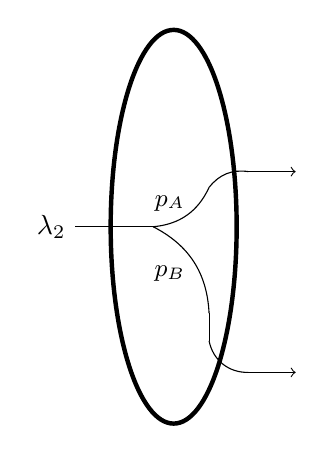
\begin{tikzpicture}
            \draw[ultra thick] (0.75,2) ellipse (0.8cm and 2.5cm);
            % \draw (0,0) -- ++(1.5cm,0) -- ++(0,4cm) -- ++(-1.5cm,0) -- ++ (0, -4cm);
            \draw[-] (0.5, 2) -- ++(-1, 0) node[left] {\(\lambda_2\)};
            
            % p_A line
            \path (0.49, 2) edge [bend right=30] (1.2, 2.5);
            \path (1.2, 2.5) edge [bend left=30] (1.7, 2.7);
            \draw[->] (1.7, 2.7) -- ++(0.6, 0.);
            
            % p_B
            \path (0.49, 2) edge [bend left=30] (1.2, 0.9);
            \draw[-] (1.2, 0.9) -- (1.2, 0.55);
            \path (1.2, 0.55) edge [bend right=40] (1.7, 0.15);
            \draw[->] (1.7, 0.15) -- ++(0.6, 0.);

            \node at (0.7, 2.3) {\small{\( p_A \)}};
            \node at (0.7, 1.4) {\small{\( p_B \)}};
        \end{tikzpicture}
    \end{minipage}
    \begin{minipage}{.55\textwidth}
        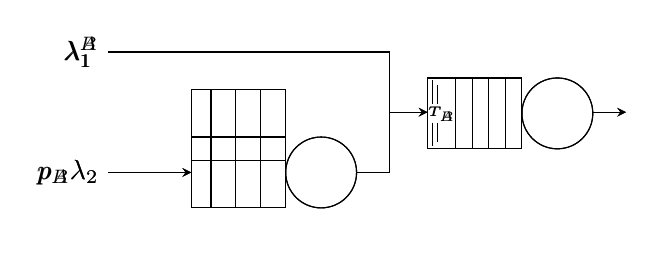
\begin{tikzpicture}[>=stealth, scale=0.6] %arrow type
            % Difference between the two queue diagrams
            \tikzmath{
                let \diff = -4.5cm;
            }

            % the rectangle with vertical lines (Queue 1)
            \draw (0,0) -- ++(2cm,0) -- ++(0,-1.5cm) -- ++(-2cm,0);
            \foreach \i in {1,...,3, 3.8}
            \draw (2cm-\i*15pt,0) -- +(0,-1.5cm);
            
            % the circle (Queue 1)
            \draw (2.75,-0.75cm) circle [radius=0.75cm];
    
            % the rectangle with vertical lines (Queue 2)
            \draw (5,1.25) -- ++(2cm,0) -- ++(0,-1.5cm) -- ++(-2cm,0);
            \foreach \i in {1,...,4, 5.7}
            \draw (7cm-\i*10pt,1.25) -- +(0,-1.5cm);

            % The two vertical lines at the very start of Queue 2 
            \draw (7cm-54pt, 1.2cm) -- +(0,-0.5cm);
            \draw (7cm-54pt, 0.3cm) -- +(0,-0.5cm);        
            \draw (7cm-51pt, 1.1cm) -- +(0,-0.4cm);
            \draw (7cm-51pt, 0.3cm) -- +(0,-0.4cm);
    
            % The label between the lines for T
            \node[anchor=north] at (5.3, 0.84) {\tiny{\( T_A \)}};

            % the circle (Queue 2)
            \draw (7.75,0.5) circle [radius=0.75cm];
    
            % the arrows and labels (Queue 1+2)
            \draw[->] (8.5,0.525) -- +(20pt,0);
            \node[align=center] at (1cm,-2cm) {};
            \node[align=center] at (6cm,-0.75cm) {};
            
            % Ambulance lines
            \draw[<-] (0,-0.75) -- +(-50pt,0) node[left] {\( p_A \lambda_2 \)};
            \draw[-] (3.5,-0.75) -- +(20pt,0);
            \draw (4.2, 0.525) -- (4.2, -0.75);

            % Others lines
            \draw (4.2, 1.8) -- +(-169.5pt,0) node[left] {\( \lambda_1^A \)};
            \draw (4.2, 1.8) -- (4.2, 0.525);
            \draw[->] (4.2, 0.525) -- (5, 0.525);

            % the rectangle with vertical rules (Queue 1)
            \draw (0, \diff) -- ++(2cm,0) -- ++(0,-1.5cm) -- ++(-2cm,0);
            \foreach \i in {1,...,3, 3.8}
            \draw (2cm-\i*15pt,\diff) -- +(0,-1.5cm);
            
            % the circle (Queue 1)
            \draw (2.75,\diff - 0.75cm) circle [radius=0.75cm];
    
            % the rectangle with vertical rules (Queue 2)
            \draw (5,\diff + 1.25cm) -- ++(2cm,0) -- ++(0,-1.5cm) -- ++(-2cm,0);
            \foreach \i in {1,...,4, 5.7}
            \draw (7cm-\i*10pt,\diff + 1.25cm) -- +(0,-1.5cm);

            % The two vertical lines at the very start of Queue 2 
            \draw (7cm-54pt,\diff + 1.2cm) -- +(0,-0.5cm);
            \draw (7cm-54pt,\diff + 0.3cm) -- +(0,-0.5cm);        
            \draw (7cm-51pt,\diff + 1.1cm) -- +(0,-0.4cm);
            \draw (7cm-51pt,\diff + 0.3cm) -- +(0,-0.4cm);

            % The label between the lines for T
            \node[anchor=north] at (5.3, \diff + 0.84cm) {\tiny{\( T_B \)}};

            % the circle (Queue 2)
            \draw (7.75,\diff + 0.5cm) circle [radius=0.75cm];
    
            % the arrows and labels (Queue 1+2)
            \draw[->] (8.5, \diff + 0.525cm) -- +(20pt,0);
            \node[align=center] at (1cm,\diff-2cm) {};
            \node[align=center] at (6cm,\diff-0.75cm) {};
            
            % Ambulance lines
            \draw[<-] (0, \diff - 0.75cm) -- +(-50pt,0) node[left] {\( p_B \lambda_2 \)};
            \draw[-] (3.5, \diff - 0.75cm) -- +(20pt,0);
            \draw (4.2, \diff + 0.525cm) -- (4.2, \diff - 0.75cm);

            % Others lines
            \draw (4.2, \diff + 1.8cm) -- +(-169.5pt,0) node[left] {\( \lambda_1^B \)};
            \draw (4.2, \diff + 1.8cm) -- (4.2, \diff + 0.525);
            \draw[->] (4.2, \diff + 0.525cm) -- (5, \diff + 0.525cm);
        \end{tikzpicture}
    \end{minipage}
    \caption{Queue}
    \label{fig:diagram_of_game_theoretic_model}
\end{figure}

The queueing systems of the hospitals are designed in such a way where they can
accept two types of individuals (section \ref{sec:queueing_model}). 
Each hospital may then choose to block type 2 individuals 
when the hospital reaches a certain capacity. 
The strategy sets for each hospital is the set 
\( \{T \in \mathbb{N} \;|\; 1 \leq T \leq N\} \) where \(N \in\{N_A, N_B\}\) are 
the total capacities of hospitals \(A\) and \(B\). We denote the chosen actions 
from the strategy set as \(T_A, T_B\) and call these \textit{threshold}s.

Both hospitals follow a queueing model with two waiting spaces for 
individuals. 
The first waiting space (i.e. the waiting space of the hospital) is where the 
patients queue right before receiving 
their service and has a queue capacity of \( N - C \), where \(N\) is the total 
capacity of the hospital and \(C\) is the number of healthcare 
professionals able to see them.
% TODO: Should this be healthcare professionals or available beds?
The second waiting space (i.e. the parking space for ambulances) is where 
ambulances, that are sent from the
ambulance service, stay until their patients are allowed to enter the hospital.
The parking space has a capacity of \(M\) and no servers.
This is shown diagrammatically in Figure~\ref{fig:diagram_of_queueing_system}.

Note here that both types of individuals can become lost to the system. 
An individual allocated from the ambulance service becomes lost to the system 
whenever 
an arrival occurs and the parking space is at full capacity (\(M\) 
ambulances already parked).
Similarly, type 1 individuals get lost whenever they arrive at the waiting 
space of the hospital and it is at full capacity (\(N - C\) individuals already
waiting).

Following this queuing model, the two queueing systems' choice of strategy will 
then rely solely on satisfying their own 
objective, which is to satisfy:

\begin{equation}
    P(W < t) \geq \hat{P}
\end{equation}

where \(W\) is the waiting time of a potential individual, \(t\) is the time 
target and \(\hat{P}\) is the percentage of individuals need to be within that 
target. 
There are numerous objective functions that can be used to capture this 
behaviour. 
For example one approach is to use the threshold that maximises the probability 
that 
the mean waiting is more than the target time, and completely ignore the 
percentage goal \(\hat{P}\).

\begin{equation}
    \arg \max_{T_i} \quad P(W_i < t)
\end{equation}

A more sophisticated objective function would be to get the proportion 
of individuals as close to the percentage aim. 
In other words, to find the threshold that minimises the difference between the 
probability and the percentage goal (or maximise its negation).

% TODO: Maybe only this equation is needed here. Remove the previous two?
\begin{equation}\label{eq:obj_queueing_systems}
    \arg \max_{T_i} \quad -\left( \hat{P} - P(W_i < t) \right)^2
\end{equation}

The third player, the ambulance service, has their own choices to make and 
their own 
goals to satisfy.
The strategy set of the third player is the proportion \(0 \leq p_A \leq 1\) of 
individuals to send to hospital A.
Similarly the proportion of individuals to send to hospital B is given by
\(p_B = 1 - p_A\).
In addition, the ambulance service aims to minimise any potential blockages
that may occur, given the pair of thresholds chosen by the two hospitals.
Thus, its objective is to minimise the blocked time of the individuals 
(\(B_A\) and \(B_B\))
that they send to hospitals \(A\) and \(B\).
Apart from the time being blocked, an additional aspect that may affect the 
decision of the distributor is the proportion of lost individuals 
\(L_A\) and \(L_B\).
Equation \ref{eq:obj_distributor} can be used to capture a mixture 
between the two objectives \(L_i\) and \(B_i\) where \(i \in \{A, B\}\):
\begin{equation}\label{eq:obj_distributor}
    (p_A, p_B) \quad s.t. \quad 
    \alpha L_A(p_A) + (1 - \alpha) B_A(p_A) = 
    \alpha L_B(p_B) + (1 - \alpha) B_B(p_B)
\end{equation}

Here, \(\alpha\) represents the ``importance'' of each objective,
where high \(\alpha\) indicates a higher weight on the proportion of lost 
individuals and smaller \(\alpha\) a higher weight on the time blocked. 

Using either equation (\ref{eq:obj_distributor}) or 
(\ref{eq:obj_queueing_systems}) gives an imperfect information extensive form 
game. 
An imperfect information game is defined as an extensive form game where some 
of the information about the game state is hidden for at least one of the 
players~\cite{Berwanger2008}. In this study the state of the problem that is
hidden is the threshold that each of the hospitals chooses to play.
In other words, each hospital chooses to play a strategy without 
knowing the other hospital's strategy.
The ambulance service then, fully aware of the chosen threshold strategies, 
distributes individuals among the two systems in order to minimise the time 
that its ambulances will be blocked. 
Figure \ref{fig:imperfect_info_game} illustrates this. 

\begin{figure}[ht]
    \centering
    \begin{tikzpicture}[-, node distance = 3cm, scale=0.8]
        \node[anchor=north](HA){\(H_A\)};
        \node[anchor=north](HA_d1) at (3, 2){.};
        \node[anchor=north](HA_d2) at (3, -2){.};
    
        \path[->] (HA) edge node {}(HA_d1);
        \path[->] (HA) edge node {}(HA_d2);
        \path (HA_d1) edge [bend left] node {}(HA_d2);
        \path (HA_d1) [dashed] edge node {}(HA_d2);
    
        \node[anchor=north](HB) at (4.1, 0){\(H_B\)};
        \node[anchor=north](HB_d1) at (6.9, 2){.};
        \node[anchor=north](HB_d2) at (6.9, -2){.};
    
        \path[->] (HB) edge node {}(HB_d1);
        \path[->] (HB) edge node {}(HB_d2);
        \path(HB_d1) edge [bend left] node {}(HB_d2);
    
        \node[anchor=north](D) at (7.8, 0){\(D\)};
        \node[anchor=north](D_d1) at (10.8, 2){.};
        \node[anchor=north](D_d2) at (10.8, -2){.};
        
        \path[->] (D) edge node {}(D_d1);
        \path[->] (D) edge node {}(D_d2);
        \path(D_d1) edge [bend left] node {}(D_d2);
    \end{tikzpicture}
    \caption{Imperfect information Extensive Form Game between the distributor 
    and the 2 queueing systems}
    \label{fig:imperfect_info_game}
\end{figure}

Hospital \(H_A\) decides on a threshold, then the hospital \(H_B\)
chooses its own threshold, without knowing the strategy of \(H_A\), and finally
the ambulance service makes its choice. 
Note here that the dotted line represents the
fact that \(H_B\) is unaware of the state of the game when making its own 
decisions. 

From equation \ref{eq:obj_queueing_systems} the utilities of the
hospitals can be formulated.
The 2-player normal form game between the two hospitals is defined by:
\begin{itemize}
    \item \textbf{Players}: Hospitals \(H_A\) and \(H_B\)
    \item \textbf{Strategy spaces}: \(T_A = \{1, 2, \dots, N_A\}, 
    T_B = \{1, 2, \dots, N_B\}\)
    \item \textbf{Utilities}:    
    \begin{equation} \label{eq:payoff_entry}
        U_{T_A, T_B}^i = 1 - \left( \hat{P} - P(W_i < t) \right)^2 \quad
        \textbf{where } i \in \{A, B\}
    \end{equation}
\end{itemize}

Consequently, the payoff matrices of the game can be populated by these 
utilities:

\begin{equation} \label{eq:payoff_matrices}
    A = 
    \begin{pmatrix}
        U_{1,1}^A & U_{1,2}^A & \dots & U_{1,N_B}^A \\
        U_{2,1}^A & U_{2,2}^A & \dots & U_{2,N_B}^A \\
        \vdots & \vdots & \ddots & \vdots \\
        U_{N_A,1}^A & U_{N_A,2}^A & \dots & U_{N_A,N_B}^A \\
    \end{pmatrix}, \,
    B = 
    \begin{pmatrix}
        U_{1,1}^B & U_{1,2}^B & \dots & U_{1,N_B}^B \\
        U_{2,1}^B & U_{2,2}^B & \dots & U_{2,N_B}^B \\
        \vdots & \vdots & \ddots & \vdots \\
        U_{N_A,1}^B & U_{N_A,2}^B & \dots & U_{N_A,N_B}^B \\
    \end{pmatrix}
\end{equation}

Based on the choice of strategy of these two hospitals, the ambulance service 
will then make their own choice of the proportion of individuals to send to
each system.


\subsection{Building the game}\label{sec:methodology}

The problem defined in this section describes a normal-form
game between the decision makers of two hospitals and a third player, the 
ambulance service, that 
decides how to distribute individuals to the two systems.
The strategy space of the two hospitals is defined as the possible values
that the threshold parameter can take \(T_i \in [1, N_i]\).
Then, the ambulance service has to decide on the proportion of individuals to 
send to 
each hospital \(p_A \text{ and } p_B\), where \(p_A, p_B \in [0, 1] \)
and \(p_A + p_B = 1\).
In practice this would correspond to a learned behaviour through experience of
waiting at each hospital.
Figure \ref{fig:imperfect_info_game} 
shows a diagrammatic representation of the game to be played and the decisions 
to be made.
As described in section \ref{sec:model_overview}, hospital \(A\) decides
on a strategy and at the same time, hospital \(B\) chooses its own 
threshold but unaware of the first hospital's choice.
Finally, the ambulance service makes its choice based on the strategies that the 
hospitals chose to play. 

The utilities to each player can be represented by 3 matrices; the two payoff 
matrices of the normal form game and the routing matrix.
The payoff matrices and their utilities are defined by equations 
(\ref{eq:payoff_entry}) and (\ref{eq:payoff_matrices}).

The routing matrix holds the values \((p_A, p_B)\) which are the proportion 
of ambulance patients to send to queueing systems \(A\) and \(B\).
Each pair \((p_A, p_B)\) can be calculated using equation 
(\ref{eq:obj_distributor}) and is essentially
a best response to the actions of the hospitals.
Thus, using equation (\ref{eq:obj_distributor}) for all possible sets of 
thresholds we can get the full routing matrix that consists of the proportions
to send to hospital A (\(p_A\)) and to hospital B (\(p_B\)).

\begin{equation}\label{eq:routing_matrix}
    R = 
    \begin{pmatrix}
        (p_{1,1}^A, p_{1,1}^B) & (p_{1,2}^A, p_{1,2}^B) & \dots & 
        (p_{1,N_B}^A, p_{1,N_B}^B) \\
        (p_{2,1}^A, p_{2,1}^B) & (p_{2,2}^A, p_{2,2}^B) & \dots & 
        (p_{2,N_B}^A, p_{2,N_B}^B) \\
        \vdots & \vdots & \ddots & \vdots \\
        (p_{N_A,1}^A, p_{N_A,1}^B) & (p_{N_A,2}^A, p_{N_A,2}^B) & \dots & 
        (p_{N_A,N_B}^A, p_{N_A,N_B}^B) \\
    \end{pmatrix}
\end{equation}

Note that since \(p_{i,j}^A + p_{i,j}^B = 1\) the routing matrix needs only to
store one of the two values; either \(p_{i,j}^A\) or \(p_{i,j}^B\).
Thus, the routing matrix \(R\) can be simplified to:

\begin{equation}\label{eq:routing_matrix_simplified}
    R = 
    \begin{pmatrix}
        p_{1,1}^A & p_{1,2}^A & \dots & p_{1,N_B}^A \\
        p_{2,1}^A & p_{2,2}^A & \dots & p_{2,N_B}^A \\
        \vdots & \vdots & \ddots & \vdots \\
        p_{N_A,1}^A & p_{N_A,2}^A & \dots & p_{N_A,N_B}^A \\
    \end{pmatrix}
\end{equation}

The game can thus be partitioned into a normal form game between the
two hospitals and then finding the ambulance service's best strategy. 

Consider Figure \ref{fig:imperfect_info_game} and the flow of the game that was
described (i.e. \(H_A, H_B \rightarrow D\)).
Due to the fact that the payoff matrices \(A\) and \(B\) depend on the routing 
matrix \(R\) the entries of the matrices are calculated in a backwards way 
(\(D \rightarrow H_A, H_B\)). 
This is done using backwards induction, by first solving the game from the
ambulance's point of view and then from the hospital's point of view.
Thus, for every pair of strategies \(T_A, T_B\), the values of \(p_A\) and 
\(p_B\) that satisfy equation (\ref{eq:obj_distributor}) are found
numerically using Brent's bisection algorithm~\cite{brent1973algorithms}.
Each pair \((p_A, p_B)\) corresponds to the best response of the ambulance
service to the two hospitals' played strategies.
Finally, using the routing matrix, equation (\ref{eq:payoff_entry}) can also be
used to populate the payoff matrices of the hospitals since we now know the 
arrival rate of each hospital.

Having calculated the payoff matrices \(A\) and \(B\), several algorithms can 
be used to measure some form of the emergent behaviour.
One possibility would be to compute the Nash equilibrium
which is the point of the game were both players have no 
incentive to deviate from their played strategies \cite{kreps1989nash}.
In other words their chosen strategies are a best response to each other.
Computation of Nash equilibria can be done in a relatively efficient way using 
the Lemke Howson algorithm~\cite{LemkeHowson}.
Lemke-Howson uses best response polytopes to get one of the Nash equilibrium of
the game. 
Other algorithms exists that will compute all Nash equilibria but 
for large games the computational complexity becomes problematic.
All game theoretic calculations were done in Python using the Nashpy library 
\cite{thenashpyproject}.

Another approach to measuring emergent behaviour is to consider 
the emergence itself and not only stable end points. 
Indeed, some Nash equilibria might not arise naturally. 
Thus in order to analyse the strategies played by the two hospitals, the 
learning 
algorithm asymmetric replicator dynamics is 
used~\cite{asymmetricreplicatordynamics}.
The two hospitals are modelled as two separate populations where each 
individual in the population is assigned a strategy.
As the game progresses the proportion of each player playing each strategy 
changes based on their previous interactions.
The fitness of each strategy is defined as:

\begin{equation}\label{eq:asymmetric_fitness}
    f_x = Ay, \quad f_y = x^T B
\end{equation}

Here, \(x \in \mathbb{R}^{m \times 1} \) and
\(y \in \mathbb{R}^{n \times 1}\) correspond to the proportion of individuals 
that play each strategy in each population.
Similarly, the average fitness of each strategy is given by:
\begin{equation}
    \phi_x = f_x x^T, \quad \phi_y = f_y y
\end{equation}

The rate of change of strategy \( i \) of both types of individuals is captured 
by:
\begin{equation}
    \frac{dx}{dt}_i = x_i((f_x)_i - \phi_x), \quad \text{ for all }i
\end{equation}

\begin{equation}
    \frac{dy}{dt}_i = y_i((f_y)_i - \phi_y), \quad \text{ for all }i
\end{equation}
 
In addition to asymmetric replicator dynamics, the learning algorithms
fictitious play and stochastic fictitious play \cite{fudenberg1998theory}
were used.

\subsection{Numerical results}\label{sec:numerical_results}

This subsection aims to analyse how the gaming framework can affect the 
performance measures of the two hospitals and how to escape certain inefficient 
situations.

The most commonly used method for analysing normal form games is the Nash 
equilibrium described in section \ref{sec:methodology_nash_equilibrium}.
Consider the following game:

\begin{multicols}{3}
    \begin{itemize}
        \item \( \lambda_{1_A} \) = 1
        \item \( \mu_A \) = 2
        \item \( C_A \) = 2
        \item \( N_A \) = 10
        \item \( M_A \) = 6
        \columnbreak

        \item \( \lambda_{1_B} \) = 2
        \item \( \mu_B \) = 2.5
        \item \( C_B \) = 2
        \item \( N_B \) = 10
        \item \( M_B \) = 6
        \columnbreak

        \item \( \lambda_2 \) = 2
        \item \( R \) = 2
        \item \( \alpha \) = 0.5
    \end{itemize}
\end{multicols}

The set of possible actions to choose from for player 1 and player 2 is the
set of thresholds that the EDs can choose from: 
\begin{equation}
    T_A \in [1, N_A], \quad T_B \in [1, N_B]
\end{equation}

For this example, the only Nash equilibrium of the game is achieved when both 
players choose a threshold of \( T_A = 10, T_B = 10 \).
This means that the two players' best response to each other is to only block
ambulances when they are full. 

Nash equilibria is a theoretical measure which can be
inconsistent with intuitive notions about what should be the outcome of a 
game \cite{myerson1978refinements}.
Therefore it might not be the best way to describe human behaviour.
Since the work of Maynard Smith \cite{smith1986evolutionary}, evolutionary game 
theory gives the tools for the emergence of stable behaviour.
One such model that allows for asymmetric payoffs, as is the case above, is 
replicator dynamics described in Section 
(\ref{sec:methodology_learning_algorithms}).
Stable outcomes of this algorithm will correspond to a subset of Nash
equilibria but more importantly, will give a model of emergent behaviour. 

The use of a learning algorithm allows to investigate, not only the outcome of 
the game, but also how that outcome is reached.
Consider Figure \ref{fig:ard_by_itself}. 
By running asymmetric replicator dynamics on the system the behaviour that 
emerges can be observed.
It can be seen that for this particular set of parameters the strategies of 
the two hospitals converge over time. 
Both hospital 1 (row player) and hospital 2 (column player) seem to be playing 
the same strategy \(s_{10}\) which indicates that thresholds \(T_A = 10\) and 
\(T_B = 10\) are played.
What is more important in this example is how the two hospitals reached these
decisions which also highlights the importance of using a learning algorithm.
Hospital 2 is able to reach the decision in a short amount of time while 
hospital 1 takes longer and goes through numerous strategies to get there.

\begin{figure}[H]
    \centering
    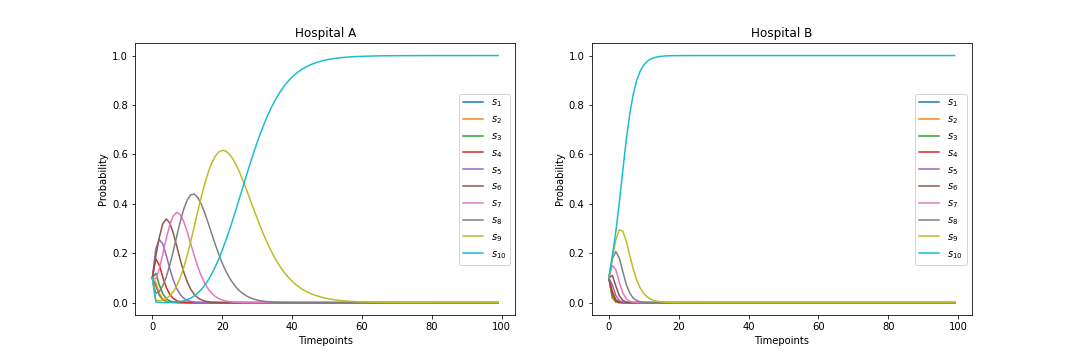
\includegraphics[scale=0.4, trim=120 0 120 0]{imgs/asymmetric_rd/asymmetric_rd.png}
    \caption{Asymmetric replicator dynamics run}
    \label{fig:ard_by_itself}
\end{figure}

In order to analyse how efficient the strategies played at every iteration are, 
the concept of the price of anarchy is used.
Price of anarchy is a measure that is used to quantify the efficiency of a
behaviour \cite{roughgarden2005selfish}.
In other words the price of anarchy is the worst-case equilibria measure and it 
is defined as:

\begin{equation}\label{eq:general_price_of_anarchy}
    \text{PoA} = \frac{\max_{s \in E} F(s)}{\min_{s \in S} F(s)}
\end{equation}

Here, \(S\) is the set of all sets of strategies \((s_A, s_B)\), \(E\) is the 
set of all possible sets of equilibria and \(F\) is the cost function to 
measure the efficiency for. 

To study the efficiency of the strategies being played, a new concept is 
introduced that considers the ratio between each hospital's best achievable 
blocking time and the one that is being played.
This new concept is defined as the compartmentalised price of anarchy of the 
players of the game and is defined as \(PoA_i(\tilde{s})\), where 
\(i \in \{A, B\}\) to distinguish among the two players/hospitals where 
\(\tilde{s}\) is the strategy that is being played by player \( i \). 
The compartmentalised price of anarchy aims to measure inefficiencies in the 
model.
The \(PoA\) for the blocking time of player \(i\) for strategy \(\tilde{s}\) 
is given by:

\begin{equation}\label{eq:poa_compartmentalised}
    PoA_{i}(\tilde{s}) = \frac{B_i(\tilde{s})}{\min_{s \in S_i} B_i(s)}
\end{equation}

Consider a game with two smaller (lower \( N_i, M_i \)) and busier (higher 
\(\lambda_{1_i} \) and \(\lambda_2\)) hospitals with the following set of 
parameters:

\begin{multicols}{3}
    \begin{itemize}        
        \item \( \lambda_{1_A} \) = 4.5
        \item \( \mu_A \) = 2
        \item \( C_A \) = 3
        \item \( T_A \in [1, N_A] \) 
        \item \( N_A \) = 6
        \item \( M_A \) = 5

        \columnbreak
        \item \( \lambda_{1_B} \) = 6
        \item \( \mu_B \) = 3
        \item \( C_B \) = 2
        \item \( T_B \in [1, N_B] \)
        \item \( N_B \) = 7
        \item \( M_B \) = 4
        
        \columnbreak
        \item \( \lambda_2 \) = 10.7
        \item \( R \) = 2
        \item \( \alpha \) = 0.9
    \end{itemize}
\end{multicols}

\textbf{Initial scenario:}
Using equation (\ref{eq:poa_compartmentalised}) and asymmetric replicator 
dynamics, the emergent behaviour can be measured and the compartmentalised price 
of anarchy at every iteration for both players.
Figure \ref{fig:ard_original} shows the strategies that are being played and 
the values of \(PoA_A(s)\) and \(PoA_B(s)\) for all iterations of the 
learning algorithm until it reaches an evolutionary stable pair of strategies.

\begin{figure}[H]
    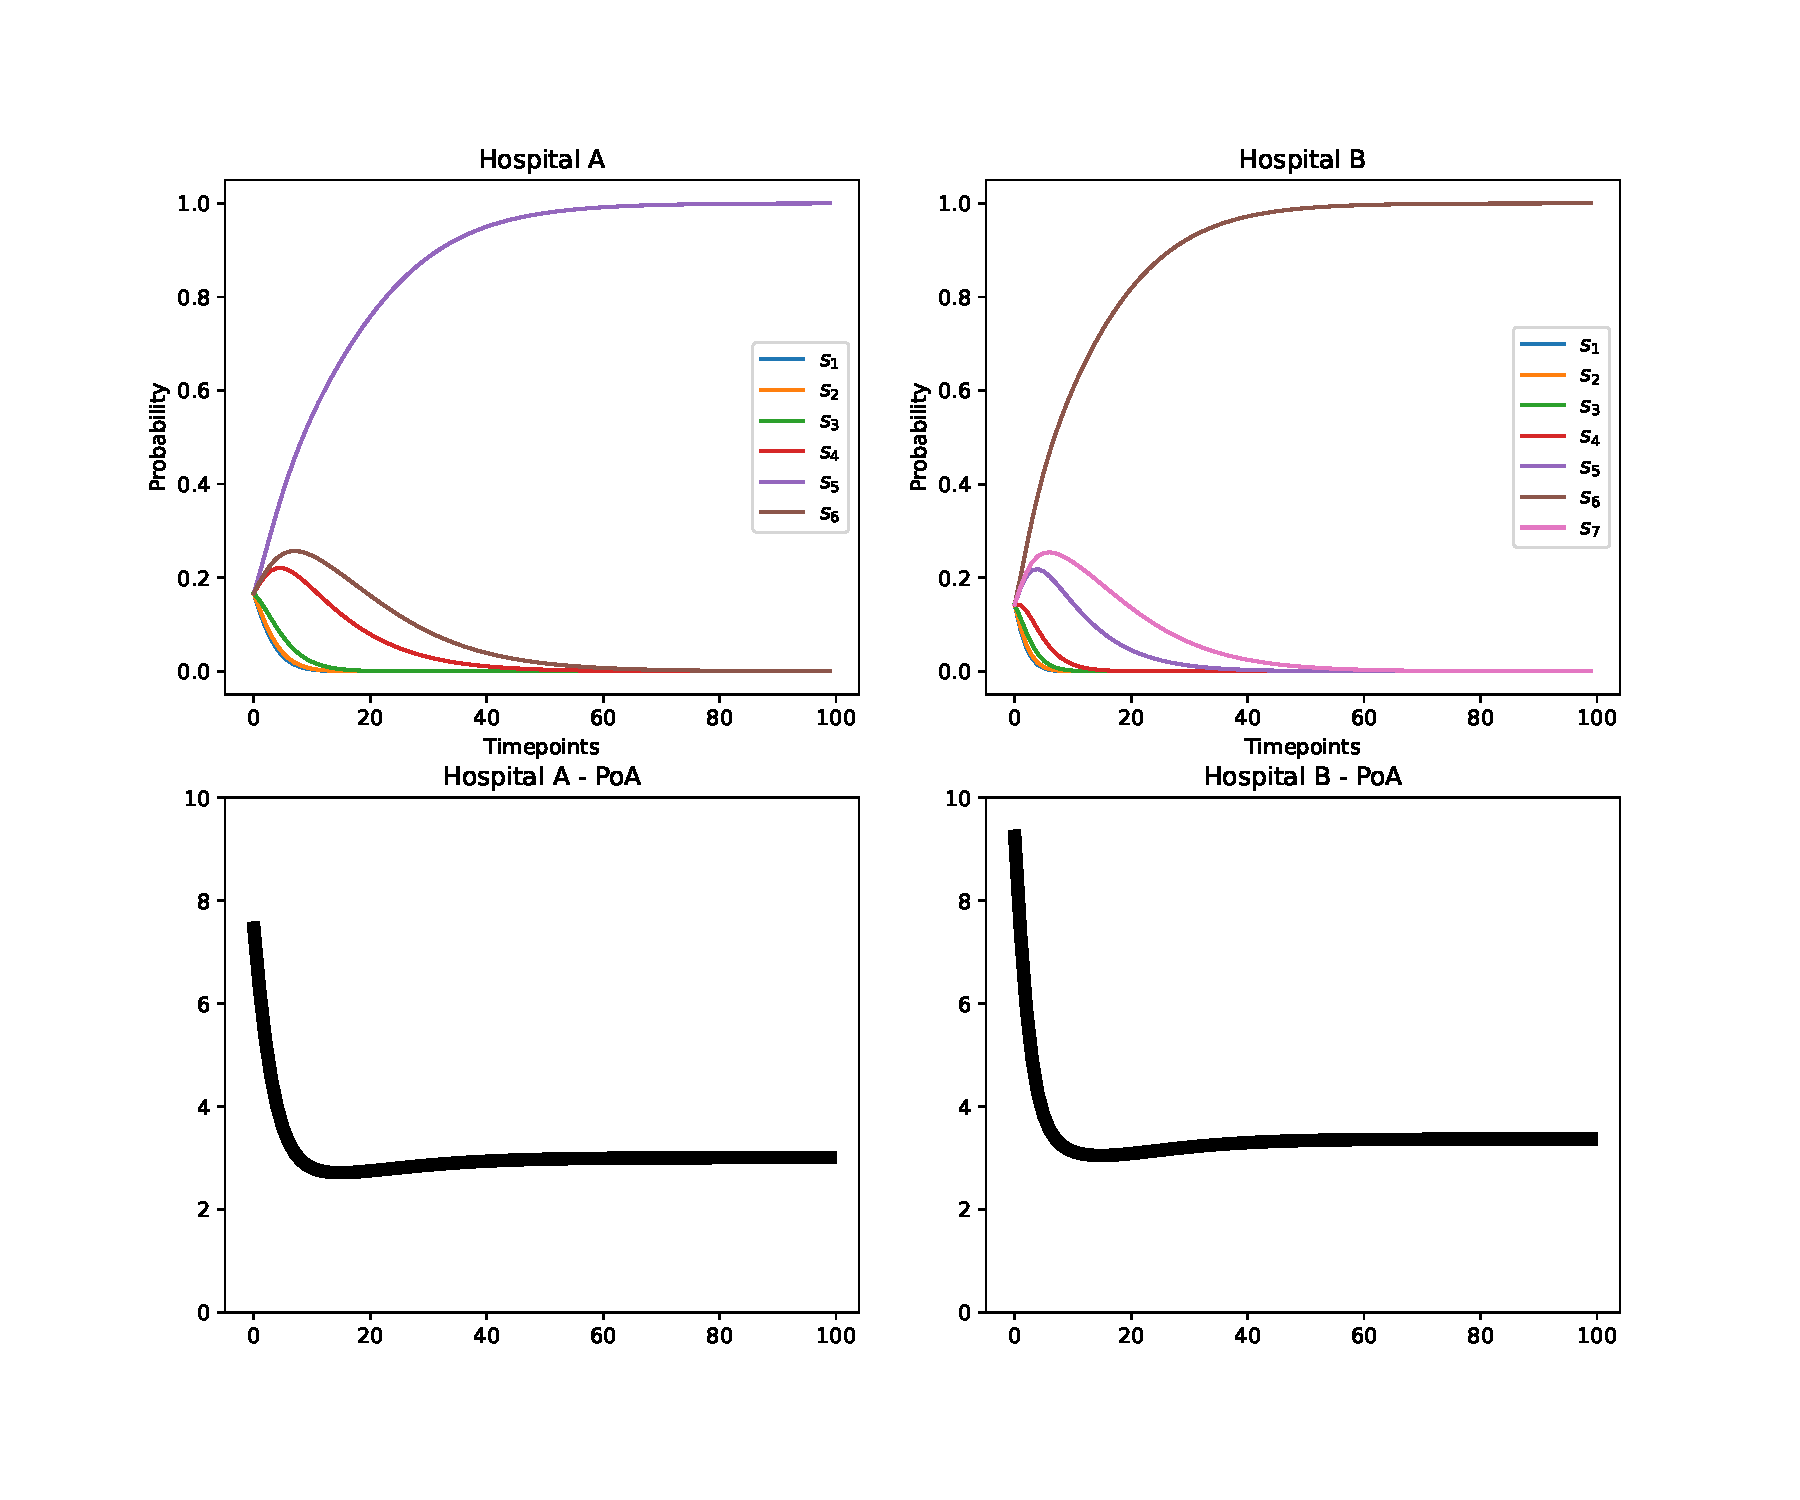
\includegraphics[width=\textwidth]{imgs/asymmetric_rd_and_PoA/asymmetric_original.pdf}
    \caption{The strategies played when running asymmetric replicator dynamics
    along with the compartmentalised price of anarchy of the blocking time at
    each iteration of the learning algorithm}
    \label{fig:ard_original}
\end{figure}

The learning algorithm reaches a stable pair of 
strategies where \(T_A = 5\) and \(T_B = 6\). After a number of iterations the
price of anarchy for both players stabilises and barely increases until the 
final iteration. 

\textbf{Increasing \(\lambda_2\):}
Figure \ref{fig:ard_lambda_2} shows a similar run of the
algorithm but when the strategies begin to stabilise an increase in the
arrival rate of ambulances occurs (i.e \( \lambda_2 = 24 \)).


\begin{figure}[H]
    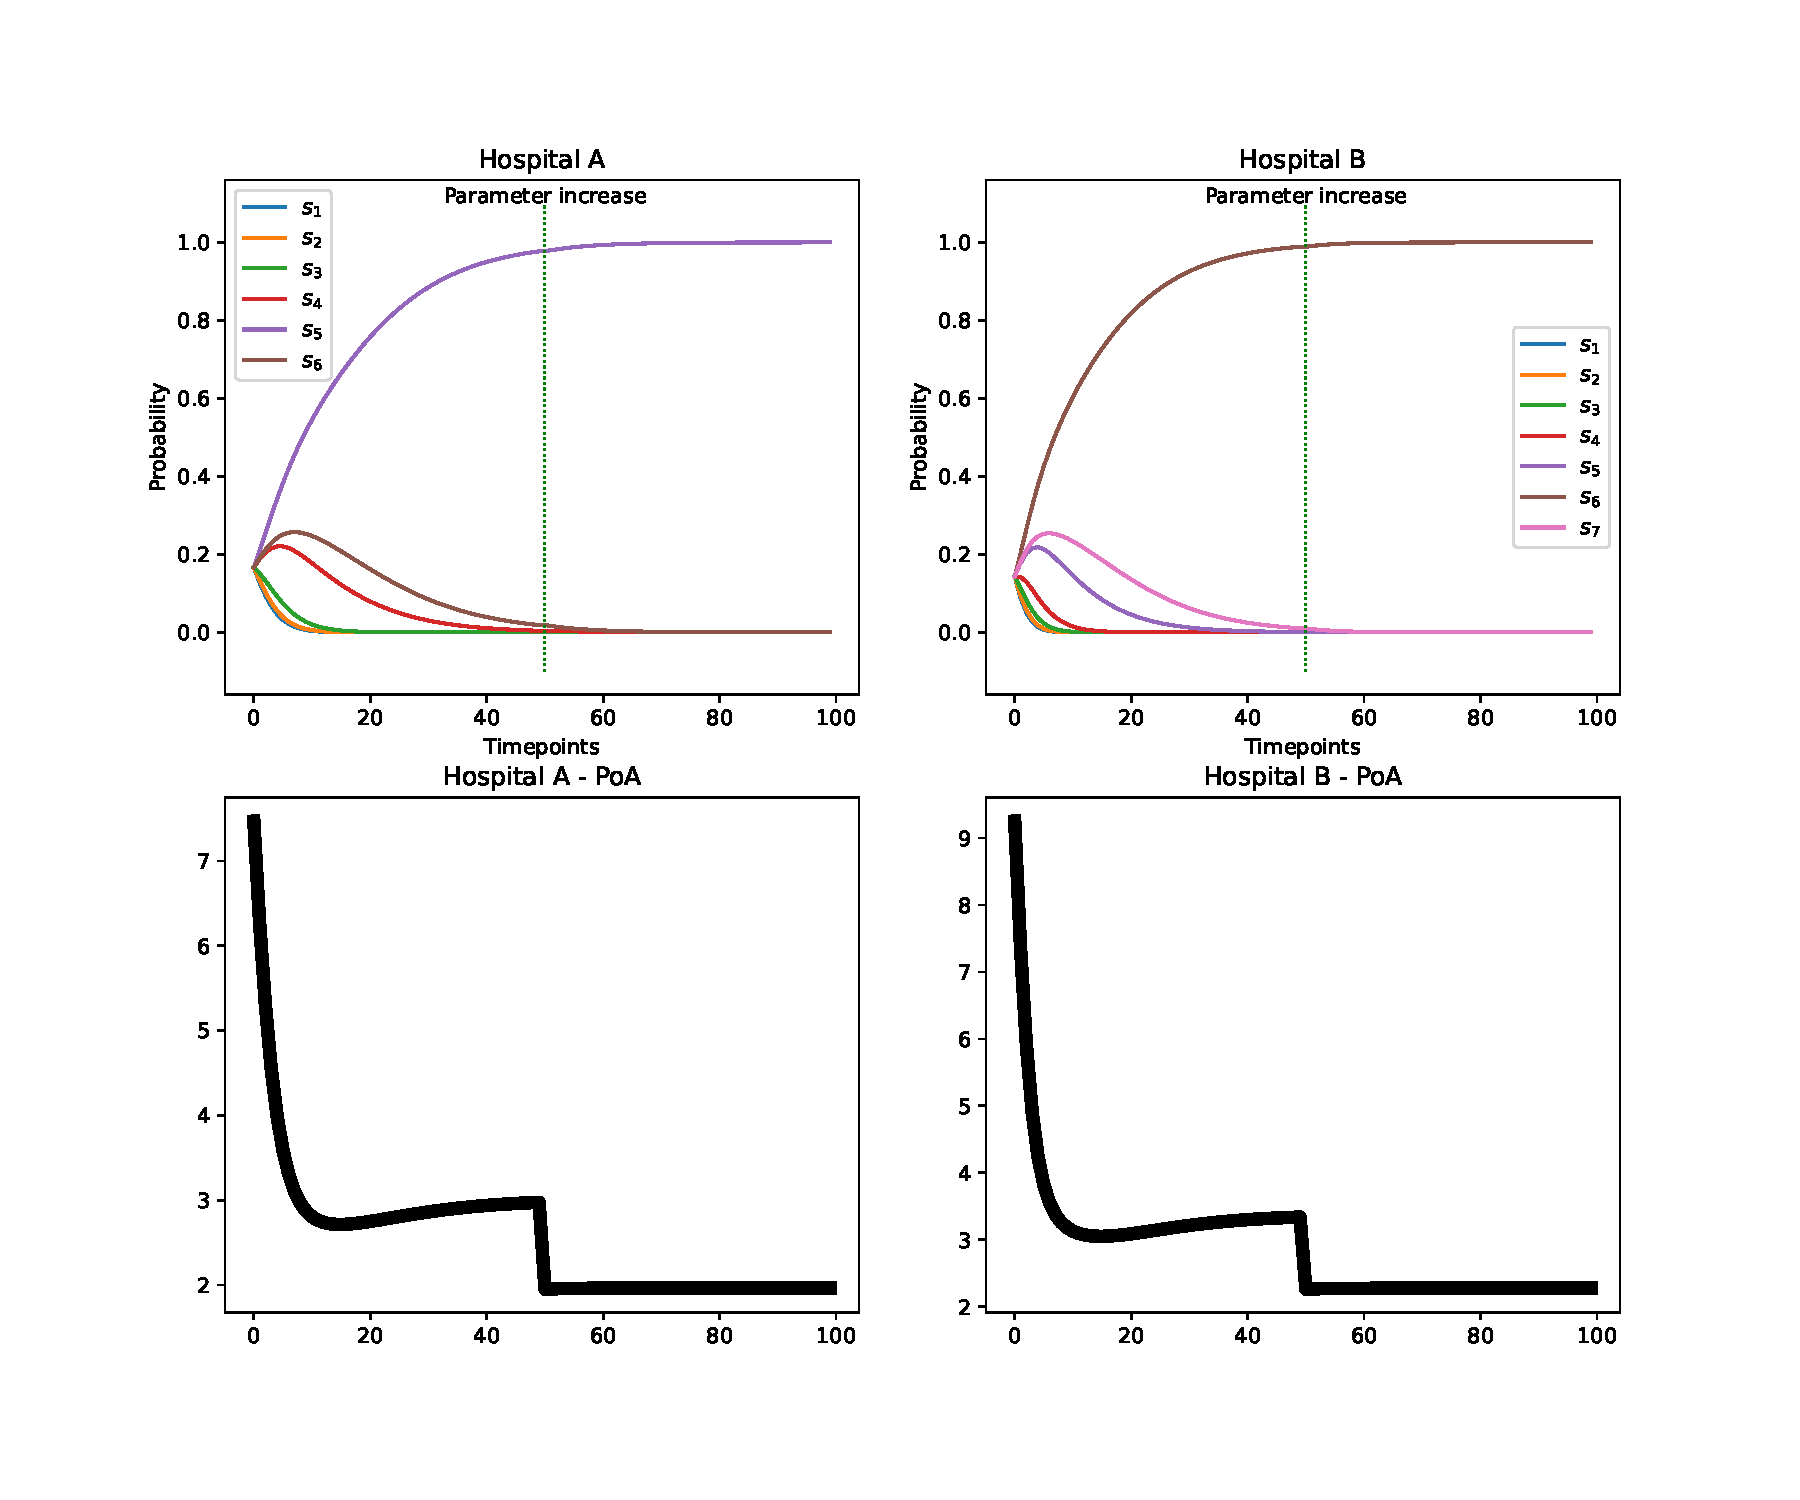
\includegraphics[width=\textwidth]{imgs/asymmetric_rd_and_PoA/asymmetric_flooding.pdf}
    \caption{The strategies played when running asymmetric replicator dynamics
    along with the compartmentalised price of anarchy of the blocking time at
    each iteration of the learning algorithm. After a number of iterations the 
    arrival rate of ambulance patients is significantly increased to flood the
    system completely \( \lambda_2 = 24 \).}
    \label{fig:ard_lambda_2}
\end{figure}


By increasing \(\lambda_2\) there is no change as to how players behave
(\(T_A = 5, T_B = 6\)), but the efficiency of the system does change. 
There is a decline in the price of anarchy of the blocking time which at first 
glance indicates that upon flooding the system it becomes the loss in efficiency
due to rational individual behaviour decreases. 
This is non-sensical though.
What it really shows is that the steep increase in \( \lambda_2 \) leaves 
the system unable to cope regardless of the decisions made.

\textbf{Increasing number of servers \( C_A \) and \( C_B \):}
Figure \ref{fig:ard_num_of_servers} shows a run of asymmetric replicator 
dynamics with a change in the number of servers of the hospitals.
The number of servers are increased from \(C_A = 3, C_B = 2\) to 
\(C_A = 4, C_B = 3\).


\begin{figure}[H]
    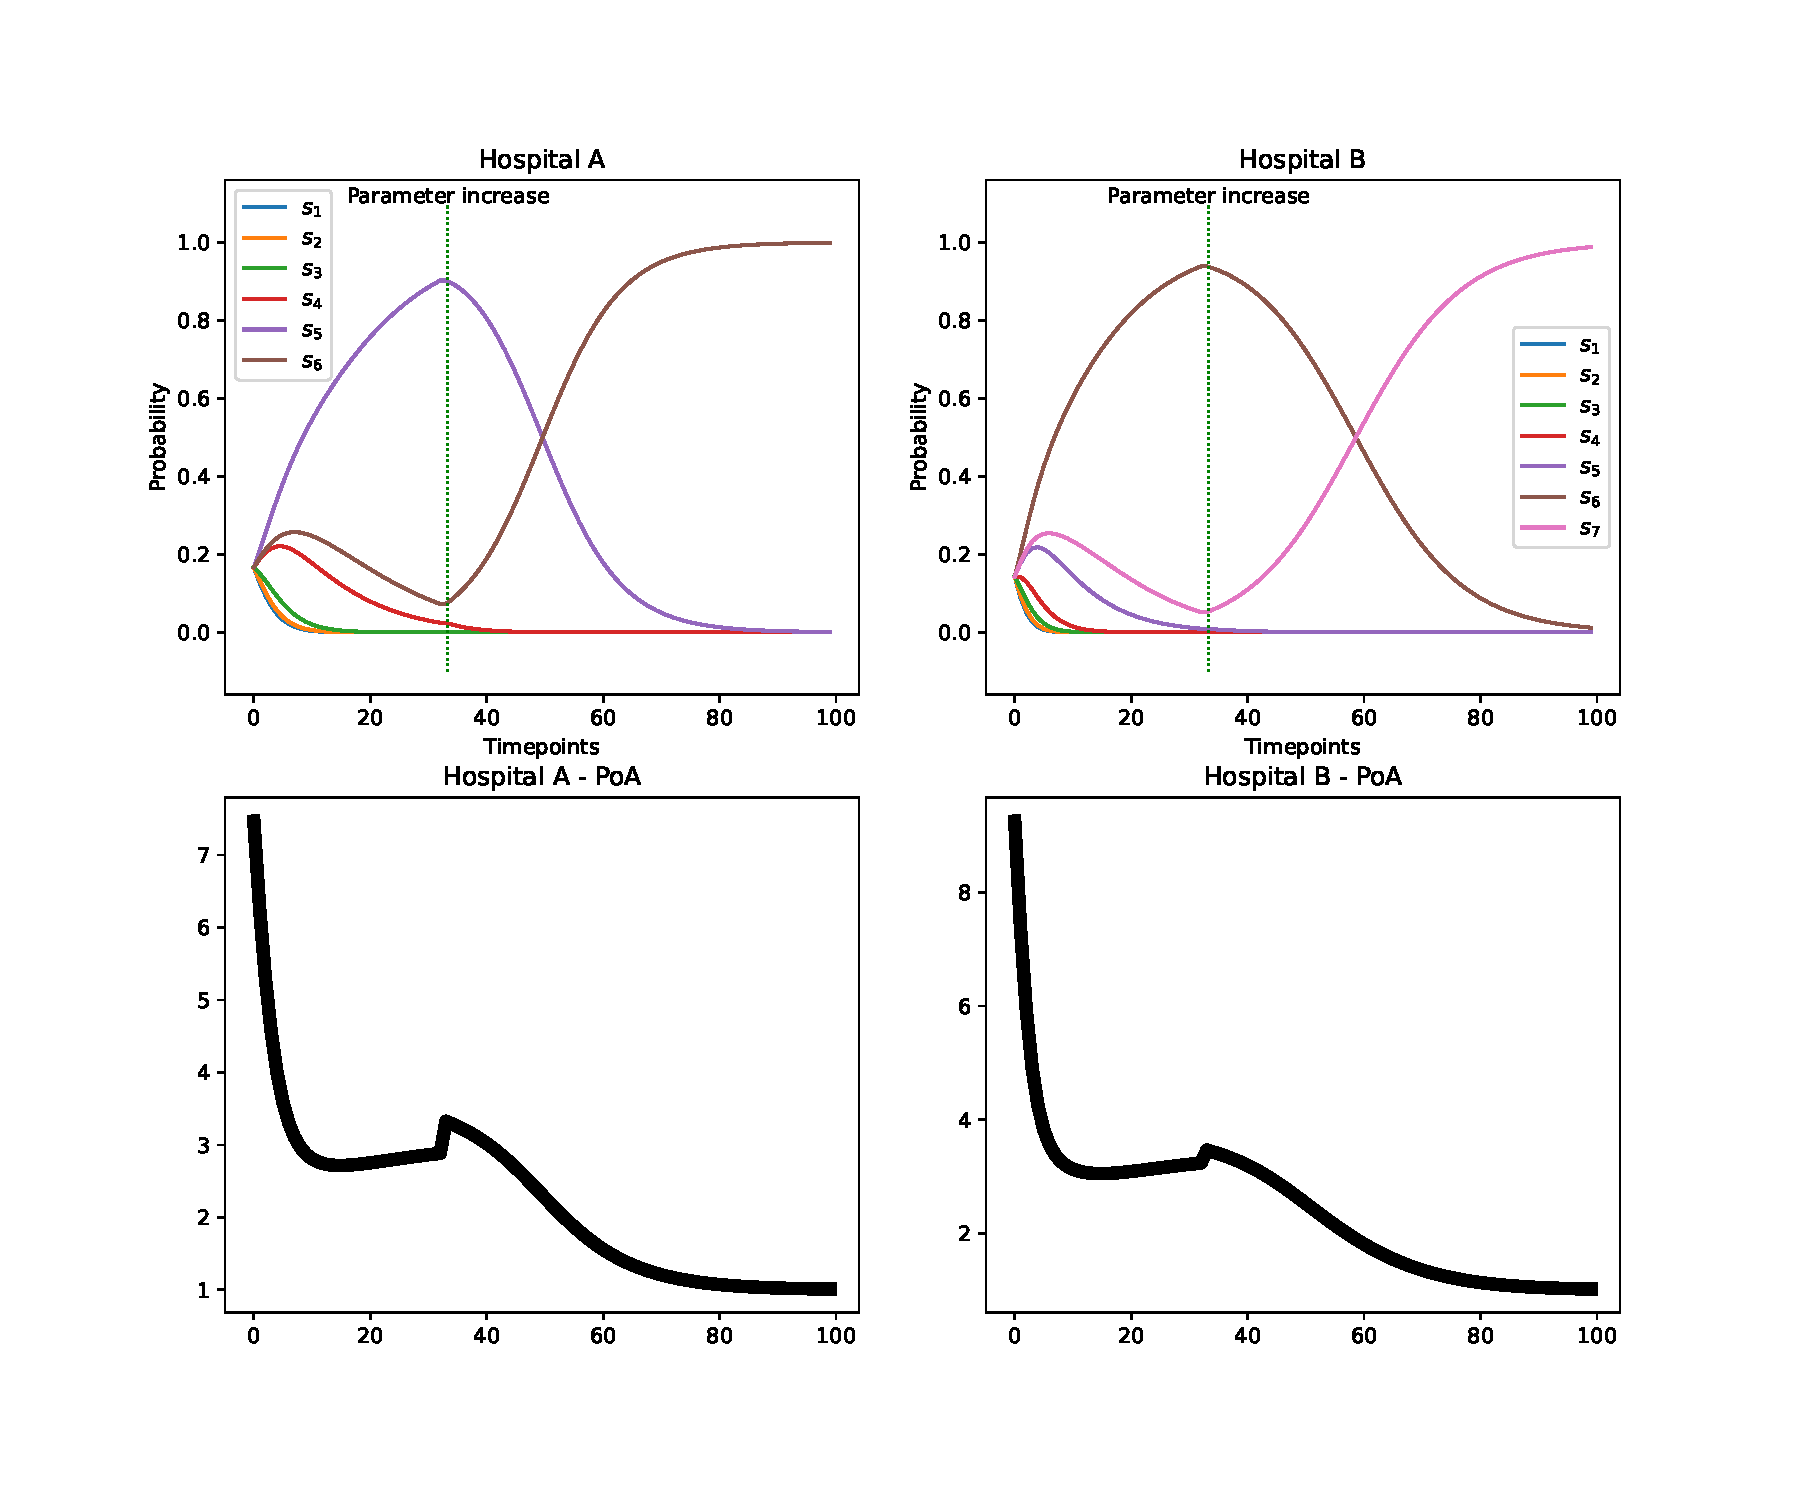
\includegraphics[width=\textwidth]{imgs/asymmetric_rd_and_PoA/asymmetric_increase_C.pdf}
    \caption{
        The strategies played when running asymmetric replicator dynamics
        along with the compartmentalised price of anarchy of the blocking time 
        at each iteration of the learning algorithm. After a number of 
        iterations the number of servers for both systems are increased by one.
    }
    \label{fig:ard_num_of_servers}
\end{figure}

In this case, both the behaviour as well as the price of anarchy change.
The players change their strategies from \(T_A = 5, T_B = 6\) to 
\(T_A = 6, T_B = 7\) and the \(PoA\) of the blocking time goes down.
By adding more resources to the models they are able to increase their 
efficiency.
Although this is a good way to escape such inefficiencies, it might not always
be cost efficient.

\textbf{Incentivising players:}
From Figures \ref{fig:ard_lambda_2} and \ref{fig:ard_num_of_servers} it can be
seen that we can change some parameters of the model to make it more efficient.
The approach used on Figure \ref{fig:ard_penalty} is slightly different than 
the previous cases.
Once the played strategies in asymmetric replicator dynamics strategies 
converge the payoff matrices of the two are scaled in such a way so that the 
utilities of the selected strategy are penalised. This corresponds to a precise
policy change where more societally beneficial behaviours are incentivised.

Matrices \(A\) and \(B\) represent the original payoff matrices while matrices
\(\tilde{A}\) and \(\tilde{B}\) represent the incentivised payoff matrices.
It can be observed that matrix \(\tilde{A}\) is a scaled version of matrix 
\(A\) only on the row that is most frequently played and similarly matrix 
\(\tilde{B}\) of matrix \(B\) only on the column that is most frequently played
(matrix \(A\): row \(5\), matrix \(B\): column \(6\), see Figure 
\ref{fig:ard_penalty}).
Note that the values of the payoff matrices only differ on the fourth digit
which is the raw utility of the strategies played.

\tiny
\begin{equation*}
    A = 
    \begin{bmatrix}
        0.9995052 & 0.9995052 & 0.9995052 & 0.9995052 & 0.9995052 
        & 0.9995052 & 0.9995052 \\
        0.99954989 & 0.99954978 & 0.99954961 & 0.99954924 & 0.99954845 
        & 0.9995466 & 0.999539 \\
        0.99968233 & 0.99968194 & 0.99968151 & 0.99968067 & 0.99967874 
        & 0.9996734 & 0.999649  \\
        0.99990299 & 0.99990245 & 0.99990189 & 0.99990081 & 0.99989832
        & 0.9998909 & 0.9998517 \\
        \color{blue}0.99999996 & \color{blue}0.99999994 & \color{blue}0.99999992 
        & \color{blue}0.99999988 & \color{blue}0.99999973 & \color{blue}0.9999989 
        & \color{blue}0.9999859 \\
        0.9998773 & 0.99987995 & 0.99988236 & 0.99988643 & 0.99989417 
        & 0.9999126 & 0.9999712
    \end{bmatrix}
\end{equation*}

\begin{equation*}
    B = 
    \begin{bmatrix}
        0.99917127 & 0.99925823 & 0.99946188 & 0.99968499 & 0.9998942 
        & \color{red}1.0 & 0.99982128 \\
        0.99917127 & 0.99925479 & 0.99945638 & 0.99968051 & 0.99989153 
        & \color{red}0.99999997 & 0.9998333  \\
        0.99917127 & 0.99924532 & 0.99943793 & 0.99966451 & 0.99988286 
        & \color{red}0.99999966 & 0.99985269 \\
        0.99917127 & 0.99924146 & 0.99942878 & 0.99965484 & 0.99987667 
        & \color{red}0.99999921 & 0.99986701 \\
        0.99917127 & 0.9992342 &  0.99941013 & 0.99963286 & 0.99986077 
        & \color{red}0.9999972 & 0.9998958  \\
        0.99917127 & 0.99921279 & 0.99934961 & 0.99954933 & 0.99978407 
        & \color{red}0.99997106 & 0.99997276 \\
    \end{bmatrix}
\end{equation*}

\begin{equation*}
    \tilde{A} = 
    \begin{bmatrix}
        0.99950518 & 0.99950518 & 0.99950518 & 0.99950518 & 0.99950518
        & 0.99950518 & 0.99950518 \\
        0.99954989 & 0.99954978 & 0.99954961 & 0.99954924 & 0.99954845
        & 0.99954656 & 0.99953879 \\
        0.99968233 & 0.99968194 & 0.99968151 & 0.99968067 & 0.99967874
        & 0.99967339 & 0.9996492  \\
        0.99990299 & 0.99990245 & 0.99990189 & 0.99990081 & 0.99989832
        & 0.9998909 & 0.99985171 \\
        \color{blue}0.99969996 & \color{blue}0.99969994 & \color{blue}0.99969992 
        & \color{blue}0.99969988 & \color{blue}0.99969973 & \color{blue}0.99969895 
        & \color{blue}0.99968586 \\
        0.9998773 &  0.99987995 & 0.99988236 & 0.99988643 & 0.99989417
        & 0.99991264 & 0.99997122 \\
    \end{bmatrix}
\end{equation*}

\begin{equation*}
    \tilde{B} = 
    \begin{bmatrix}
        0.99917127 & 0.99925823 & 0.99946188 & 0.99968499 & 0.9998942
        & \color{red}0.9997 & 0.99982128 \\
        0.99917127 & 0.99925479 & 0.99945638 & 0.99968051 & 0.99989153
        & \color{red}0.99969997 & 0.9998333 \\
        0.99917127 & 0.99924532 & 0.99943793 & 0.99966451 & 0.99988286
        & \color{red}0.99969966 & 0.99985269 \\
        0.99917127 & 0.99924146 & 0.99942878 & 0.99965484 & 0.99987667
        & \color{red}0.99969921 & 0.99986701 \\
        0.99917127 & 0.9992342 &  0.99941013 & 0.99963286 & 0.99986077
        & \color{red}0.9996972 & 0.9998958 \\
        0.99917127 & 0.99921279 & 0.99934961 & 0.99954933 & 0.99978407
        & \color{red}0.99967106 & 0.99997276 \\
    \end{bmatrix}
\end{equation*}
\normalsize


\begin{figure}[H]
    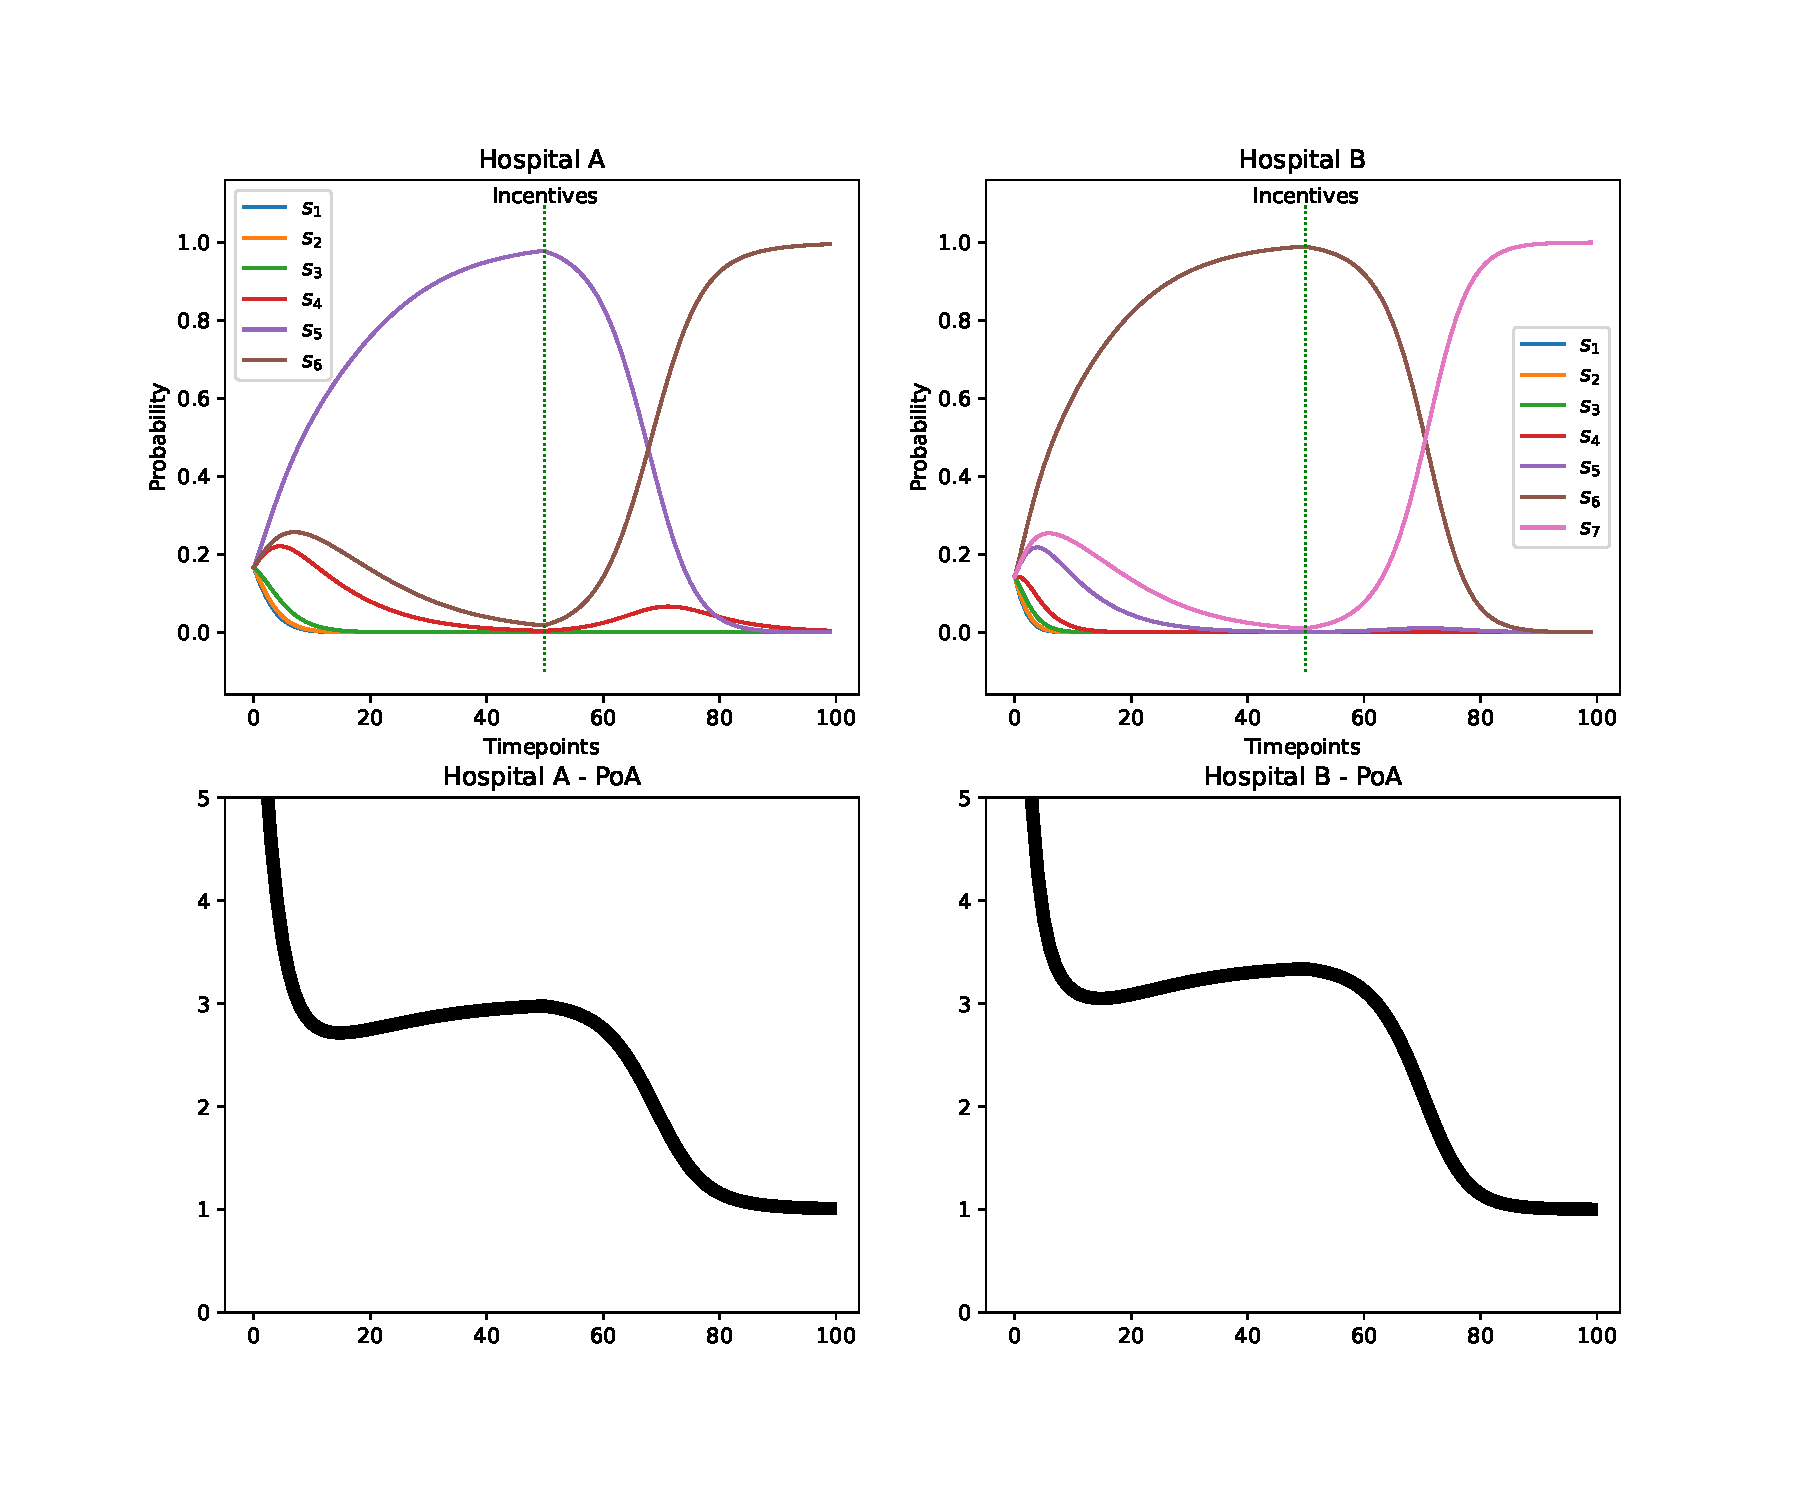
\includegraphics[width=\textwidth]{imgs/asymmetric_rd_and_PoA/asymmetric_penalty.pdf}
    \caption{
        The strategies played when running asymmetric replicator dynamics
        along with the compartmentalised price of anarchy of the blocking time 
        at each iteration of the learning algorithm. After a number of 
        iterations the most dominant strategy is being penalised.
    }
    \label{fig:ard_penalty}
\end{figure}

Figure \ref{fig:ard_penalty} shows that players start playing strategies 
\( T_A = 5\) and \( T_B = 6 \) and mid-run of the learning algorithm a penalty
is applied to these strategies on the payoff matrix.
By incentivising the players in such a way the players change their strategies 
to \(T_A = 6\) and \(T_B = 7\), and thus ambulance patients are accepted in the 
ED more often.
Hence, the \(PoA\) for both EDs is decreased, meaning that the whole system is
more efficient in terms of the blocking time.
